\chapter{Sentence Translation}
As mentioned previously, training a traditional machine translation system requires large parallel data. With cross-lingual word embedding we can already find ambiguous word translations, in this chapter I propose a simple yet effective method to improve quality of translation which starts from the word-by-word translation. We integrate additional models, such as language model of the target side and denoising neural network of the target side to produce meaningful sentence translation. Since all the our models  are trained on monolingual corpora, This  method is fully unsupervised. Such system surpasses state-of-the-art unsupervised NMT without costly iteratively training.  
\section{Context-aware Beam Search}
	\subsection{Language Model}
		Language models are widely applied in NLP tasks, they assign a probability to a sequence of words so that they can improve the quality of systems outputs like machine translation, spell correction, speech recognition and question-answering, etc.,.According to the similarity of cross-lingual word embedding, we are able to find some meaningful for translation candidates for a given word. But there are also words that actually noise in the candidates or obviously incorrect because of grammar checking. With the support of language model, we can select the most probable words given previous word translation candidates. 
		
		${N}$-gram language models use the Markov assumption to break the probability of a sentence into the product of the probability of each word given a limit history of preceding words. 
		\[ p(e_1^I) = \prod_{i=1}^{I} p(e_i| e_1, \cdots	e_{i-1}) = \prod_{i=1}^I {p(e_i | e_{i-(I-1)}, \cdots , e_{i-1})}  \] 
		
		The conditional probability can be calculated from ${N}$-gram model frequent counts:
		\[p(e_i | e_{i-(n-1)}, \cdots , e_{i-1}) = \frac{count(e_{i-(n-1)}, \cdots, e_i)}{count(e_{i-(n-1)}, \cdots, e_{i-1})} \]
		Language model can handle sparse data problem. Some words or phrases have not been seen yet in the training corpus does not mean they are not impossible. Different smoothing techniques like back-off or interpolation are implemented to assign a probability mass to unseen cases.
	\subsection{Beam Search}
	When using LM, the complexity of a search graph is exponential to the length of the given source sentence. Beam search is a heuristic search algorithm that explores a graph by expanding the most promising nodes. At each step of the search process, it will evaluate all the candidates together with the reserved translation results from last step, it will only store a predetermined number (beam size) of translations for next step. The greater the beam size is, the fewer states will be pruned. 	
	Tt is suggested to prune poor word translation candidates as soon as possible to reduce the search space and speed up the translation. 
	
	In this thesis, translation system does not handle reordering, it combines the language model and lexicon model to construct a word-by-word framework, where the output length equals that of input sentence. Since the lexicon model actually gives a cosine similarity instead of a normalized probability, we introduce weights $\lambda_{LM}$ and $\lambda_{lex}$ to scale the contribution of each of the two components:
	\[ \hat{e}_1^J = \argmax{e_1^J}{\ \prod_{i=1}^{J}} {p^{\lambda_{LM}}(e_i|e_{i-(n-1)}^{i-1}) \cdot q^{\lambda_{lex}}(f_i,e_i)}\]

 	where the lexicon score ${q(f,e) \in [0,1]}$ defined as:
 	\[q(f,e) = \frac{d(f,e)+1}{2} \]
 	${d(f,e)\in [-1,1]}$ cosine similarity between $\bm{f}$ and $\bm{e}$
	
	
	In experiments, we find linear scaling works better than others, e.g. sigmoid or softmax.
	
\section{Denoising Neural Network}
\subsection{Denoising Auto-encoder (DAE)}
	With the help of language model, we improve the quality of word-by-word translation but the results are still far from acceptable. Because of the natural defect of word-by-word translation, word sequence in translation keeps the same as in input. This is contrary to our knowledge that different languages have different grammars also sequences. We implement the sequential DAE to improve the translation output.
	
%	An autoencoder is a neural network that is trained to copy its input to the output. Autoencoders minimize the loss function like: 
%	\[ L(\bm x, g(f(\bm x))) \]
	Autoencoder is a type of neural network model used to learn efficient data coding, typically dimension reduction in an unsupervised manner. The DAE is to force the hidden layer to discover more robust features by training the autoencoder to reconstruct the input from a corrupted version. It does two things, try to encode the input and try to undo the effect of a corrupt process stochastically applied to the input. In our model, the corrupt input is the word-by-word translation and the output ought to be the standard translation with correct sequence. Since we do not have parallel data as the references. We need to model the denoising process with artificial parallel data. We design three types of noises including a novel noise type to mimic the corrupted sentence. The loss function for DAE is defined as: 
	\[ \mathcal{L}^{auto} = \mathbb{E}_{e_1^I \sim \mathcal{E}}[-\log P(e_1^I| \text{noise}(e_1^I))] \]
	where $\text{noise}(e_1^I)$ is noisy target sentences where artificial noises are added.

	
\subsection{Noise Model}
We design three types of noise to handle the fertility and reordering problem, namely reordering noise, insertion noise and deletion noise. 

%In experiments, the noise model can improve the sentence translation, but since it actually starts from the word-by-word translation, it can only deal with reordering in limited distance, cannot work for global reordering.\\

	\begin{figure}[h]
	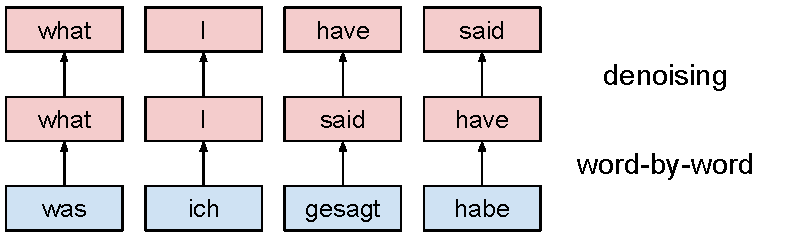
\includegraphics[width=14cm]{denoising}
	\caption{ Reordering noise}
	\centering
\end{figure}
	\textbf{Reordering Noise}\\

	The reordering problem is a common phenomenon in the word-by-word translation since the word order in source language is not the same in target language. 
	For example, in  the grammar of German, the verb is often placed at the end of the clause. 
	``um etwas zu tun". However in English, it is not the case; the corresponding translation sequence is ``to do something". The verb should always before the noun.
	In our beam search, LM only assists in choosing  more suitable word from the translation candidates, and cannot reorder the word sequence at all.
	
	For a clean sentence from the target monolingual corpora, we corrupt the word sequence by permutation operation. We limit the maximum distance between the original position and its new position.
	
	The design of reordering noise is as followed:
	\begin{enumerate}
		\item For each position ${i}$, sample an integer ${\delta_i}$ from ${[0, d_{per}]}$
		\item Add ${\delta_{i}}$ to index ${i}$ and sort ${i+\delta_{i}}$
		\item Rearrange the words to be in the new positions, to which where indices have been moved
	\end{enumerate}

	Reordering actually depends on specific language pair. The reordering noise here just models the most general case.
%	However in the experiments we found the performance of the denoising network aimed at such noise is not obvious. The Bleu score before and after the process is close.\\

	
	\textbf{Insertion Noise}\\
	\begin{figure}[ht]
	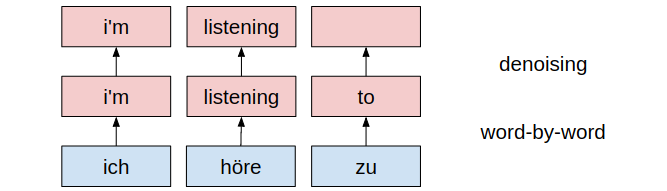
\includegraphics[width=14cm]{insertion}
	\caption{Insertion noise}
	\centering
\end{figure}	

	The word-by-word translation system predict a target word at every source position of the sentence. However,  the vocabularies of different languages are not symmetric. For example, in German, there are more compound words than that in English. So when translating between languages, there are a plenty of cases that a single word will be translated to multiple words and multiple words correspond to a single word conversely. For example: from a German sentence: ``ich höre zu" to ``i'm listening". A very frequent word ``zu" which corresponds to ``to" in English, is dropped from the sentence. The design of reordering noise is as followed:
	\begin{enumerate}	
		\item For each position ${i}$, sample a probability ${p_i \sim \textrm{Uniform}(0,1)}$
		\item If ${p_i} < p_{ins}$, sample a word ${e}$ from the most frequent ${V_{ins}}$ target words and insert it before the position${i}$
	\end{enumerate}

	We limit the insertion word in a set consisting of the top frequent word in the target language ${V_{ins}}$ \\
	
	




	\textbf{Deletion Noise}\\
	The deletion noise is just a contrary case of insertion noise.
	Because we are limited to generate only one word per source word, it is also possible that a target word in the reference is not related to any source word.  For example for ``eine der besten" the corresponding translation is ``one of the best". We need to add an extra preposition in the target sentence.  To simulate such situation, we drop some words randomly from a clean target sentence.
	
	\begin{enumerate}
		\item For each position i, sample a probability ${p_i \sim \textrm{Uniform}(0,1)}$
		\item If ${p_i} < p_{del}$, drop the word in the position i
	\end{enumerate}
	
		\begin{figure}[h]
		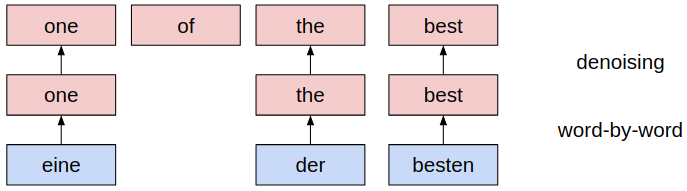
\includegraphics[width=14cm]{deletion}
		\caption{ Deletion noise}
		\centering
	\end{figure}

	
	
	
	
	
	
	
	
	
	
	
	
	
	
	
	
	
	
	
	
	
	
	
	
	
	
	
	